\chapter{Tesztelés} % Testing


%Memory leak
\section{Memóriaszivárgás}

A C++ nyelv sajátosságai közé tartozik, hogy örökölte a C nyelvből a memóriaterületekre való mutatók használatát és azok lefoglalásának és felszabadításának manuális feladatát. Memóriaszivárgásról (memory leak) akkor beszélhetünk, ha egy adott memóriaterület lefoglalásra kerül a program futása során, azonban az sosem szabadul fel, vagy túl későn. Ez hibát okozhat egy dinamikusabb memóriakezelésű környezetben, ahol sokszor hozunk létre objektumokat majd távolítjuk el őket. Amennyiben a felhasználható memória elfogy, a program futása a következő memóriahívás létrehozásakor leáll, vagy a számítógépen a többi párhuzamosan futó program futását akadályozza.

Ezen program minimális memóriaszivárgási kockázattal jár, ugyanis fix bufferekkel dolgozik és azokat a futás első szakaszában egyszer hozza létre. Ennek ellenére amennyiben egy ilyen hiba megjelenik, az biztosan mutatja hogy valami nem megfelelően működik a belső rendszerben, ezért egy tökéletes hibakezelési módszer.

A memóriaszivárgásokat manuálisan megkeresni szinte lehetetlen, amennyiben elég kis területekról van szó, hogy ne látsszon a memóriahasználati grafikonon. Ezért egy Microsoft által fejlesztett könyvtárat alkalmaztam, amely a program futásának befejeztével kilistázza a nem felszabadíott memóriaterületek címeit és azok tartalmát, amelyet segítséget nyújtanak azok megtalálásában.

A main fájlban kell importálni a könyvárat, majd a main futásának befejeztével kiiratni az esetleges hibákat.

\lstset{caption={Microsoft CRT könyvtár implementációja a rendszerben}, label=src:cpp}
\begin{lstlisting}[language={C++}]
//Memoryleak test
#ifdef _DEBUG
	#define _CRTDBG_MAP_ALLOC
	#include <stdlib.h>
	#include <crtdbg.h>
#endif // _DEBUG

//Main
int main(int argc, char* argv[])
{
	RelayResult result = MainCommandRelay::relay(argc, argv);

	#ifdef _DEBUG
		_CrtDumpMemoryLeaks();
	#endif //_DEBUG

	return static_cast<int>(result);
}
\end{lstlisting}

Látható, hogy csak akkor importáljuk a könyvtárat, amikor debug üzemmódban fordítjuk a programot, illetve a kiiratás metódusa is csak ebben az esetben lesz meghívva.

\lstset{caption={Memóriaszivárgás üzenet példa}, label=src:cpp}
\begin{lstlisting}
Detected memory leaks!
Dumping objects ->
{18} normal block at 0x0178FE61, 32 bytes long.
 Data: <                > 00 00 00 00 00 00 00 00
Object dump complete.
\end{lstlisting}






%Unit test
\section{Egységtesztelés}

A program tesztelésének a fő módszere az egységtesztelés (unit test) jelen esetben. Az egységeket a program lefutásának kis szakaszaira lehet alkalmazni, ezáltal kideríthető, hogy a hiba pontosan melyik egységből származik.

Az egységek tesztelése a Microsoft Visual Studio beépített eszközeivel történik, amelyet képesek futtatni az előre megírt tesztelő kódot és azok eredményét egy jól érthető és gyorsan áttekinthető felületen prezentálni. Erre egy külön teszt projekt lett létrehozva a program főkönyvtárában. Fontos, hogy a tesztelő helyes működéséhez a fordítási beállításoknak Debug módban kell lenniük.

A tesztek elkészítéséhez módosítanom kellett a függvények visszatérési értékén, ahogy azok megfelelően tesztelhetővé váljanak, az eredményeket ne csak a kimeneti konzolban jelenítsék meg. Ezen felül többször előfordult, hogy az OpenCL optimalizáció során hibás eredményeket generált a hash funkció, amelyeket az egységteszteknek sikerült jelezni.

\lstset{caption={A GPUController hashSingle metódusának tesztelése.}, label=src:cpp}
\begin{lstlisting}[language={C++}]
//Load
GPUController* gc = new GPUController();
gc->attachDevice({});

//Hash
Assert::AreEqual(std::string("b493d48364afe44d11c0165cf470a4164d1e2609911ef998be868d46ade3de4e"), gc->hashSingle("banana"));
Assert::AreEqual(std::string("c79c99dded78b97103916e94e5bc052d0b881ad2da896674b177bda1b1830e35"), gc->hashSingle("encloses"));
Assert::AreEqual(std::string("9c9e82db146a9bfe73b43aebfa89cd889a4fccc6fe916a66dcd497ecc4c182a2"), gc->hashSingle("enclosesHf45DD"));
Assert::AreEqual(std::string("59557cf1890bf0b7458c1e66119ab01c3a796fd09df296ef7e70745d29934777"), gc->hashSingle("ex-wethouder"));

//Length mods (4)
Assert::AreEqual(std::string("ca978112ca1bbdcafac231b39a23dc4da786eff8147c4e72b9807785afee48bb"), gc->hashSingle("a")); //1
Assert::AreEqual(std::string("961b6dd3ede3cb8ecbaacbd68de040cd78eb2ed5889130cceb4c49268ea4d506"), gc->hashSingle("aa")); //2
Assert::AreEqual(std::string("9834876dcfb05cb167a5c24953eba58c4ac89b1adf57f28f2f9d09af107ee8f0"), gc->hashSingle("aaa")); //3
Assert::AreEqual(std::string("61be55a8e2f6b4e172338bddf184d6dbee29c98853e0a0485ecee7f27b9af0b4"), gc->hashSingle("aaaa")); //0
Assert::AreEqual(std::string("ed968e840d10d2d313a870bc131a4e2c311d7ad09bdf32b3418147221f51a6e2"), gc->hashSingle("aaaaa")); //1

delete gc;
\end{lstlisting}

Látható, hogy a teszt első lépésében létrehozunk egy GPUController objektumot és rákötjük a rendszer alapértelmezett eszközére. Ezután elvégzünk egy néhány előre ismert hashelést és ellenőrizzük az eredményüket. A második részben tesztelünk különböző karakterhosszúságú sorokat, hiszen a program más ágon megy keresztül amennyiben ezek hossza maradékosan osztva 4-el különbözik.

Ez a teszt lépés a GPU oldalon épp használt hashelés helyességére fókuszál, amely különösen előnyösnek bizonyult az eszköz oldali optimalizáció közben. A többi teszt is hasonlóképp épül fel, amelyek a program működésének különböző elemeire fókuszálnak rá.
%
\begin{itemize}
    \itemsep-0.5em
    \item GPUController
        \begin{itemize}
            \item \textbf{CopyKernels} - Minden kernelkód létezik-e és a friss verziók átmásolódnak a tesztelő mappájába.
            \item \textbf{Creating Controller} - A controller helyesen létrejön-e és rá tud-e csatlakozni az alapértelmezett eszközre.
            \item \textbf{HashSingle} - Egy jelszó hashelés helyes-e.
            \item \textbf{HashSingleSalted} - Egy jelszó és salt hashelés helyes-e.
            \item \textbf{CrackSingle} - Egy jelszó feltörése helyes-e egy rövid jelszófájl használatával.
            \item \textbf{CrackSingleSalted} - Egy jelszó salt-os feltörése sikeres-e egy rövid jelszófájl használatával. Azt hogy a megadott hash salt-al van ellátva a helyesen program állapítja-e meg.
        \end{itemize}
    \item LinkedList
    \begin{itemize}
            \item \textbf{Creating} - Helyesen elkészül-e egy példány.
            \item \textbf{Filling} - Helyesen hozzáadhatók-e elemek.
            \item \textbf{Popping} - Helyesen eltávolíthatók-e elemek.
            \item \textbf{Exporting} - Helyesen exportálhatók-e az elemek egy std::vector-ba.
        \end{itemize}
\end{itemize}

A beépített tesztelő felületet a Visual Studio főablakának főmenüjében a Test > Test Explorer gombbal érhetjük el.

\begin{figure}[H]
    \centering 
    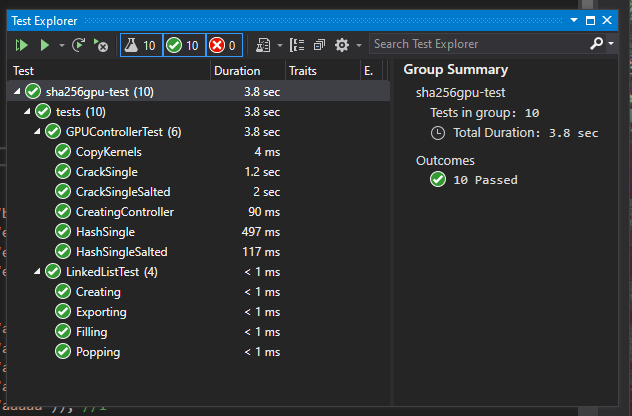
\includegraphics[width=\textwidth]{images/examples/tests.png}
    \caption{A tesztek példa futtatása.}
\end{figure}






%Big data
\section{Nagy Adattömeg}

A program egyik fő szempontja volt a skálázhatóság, ezért jól kell teljesítenie bármekkora adattömegen, lineáris teljesítményromlással. A tesztelést a 4 millió soros adatfolyam másolásával végeztem, ahol minden sor betűit véletlenszerűen összekevertem és a fájl mögé illesztettem 100-szor, minden alkalommal újra összekeverve. Ezáltal egy majdnem \num{400000000} elemű jelszó fájl jött létre, melynek lemezen elfoglalt mérete 4.367 GB.

Hibahatárnak nagyjából 5\%-ot jelöltem ki, hiszen a számítógép sosem neutrális állapotban van és ezek befolyásolhatják a futási időt. Ennek a futási ideje 98.18 szorosa volt az eredeti majdnem 4 millió elemű fájlénak, amely hibahatáron belül helyezkedik el, így látható, hogy a program futási ideje lineárisan növekszik nagyobb adatfolyamok feldolgozása esetén.